\section{Dataset Description}

We selected the \href{https://www.yelp.com/dataset}{Yelp Open Dataset}, a 8.65 GB dataset which contains a subset of businesses, user data, and reviews provided as JSON files. The dataset is made up of 6,990,280 reviews, 150,346 businesses, and 200,100 pictures (not utilized in our project) from 11 metropolitan areas. Over 1.2 million business attributes are accessible along with 908,915 tips (quick suggestions) from 1,987,897 users.

\begin{figure}[h!]
    \centering
    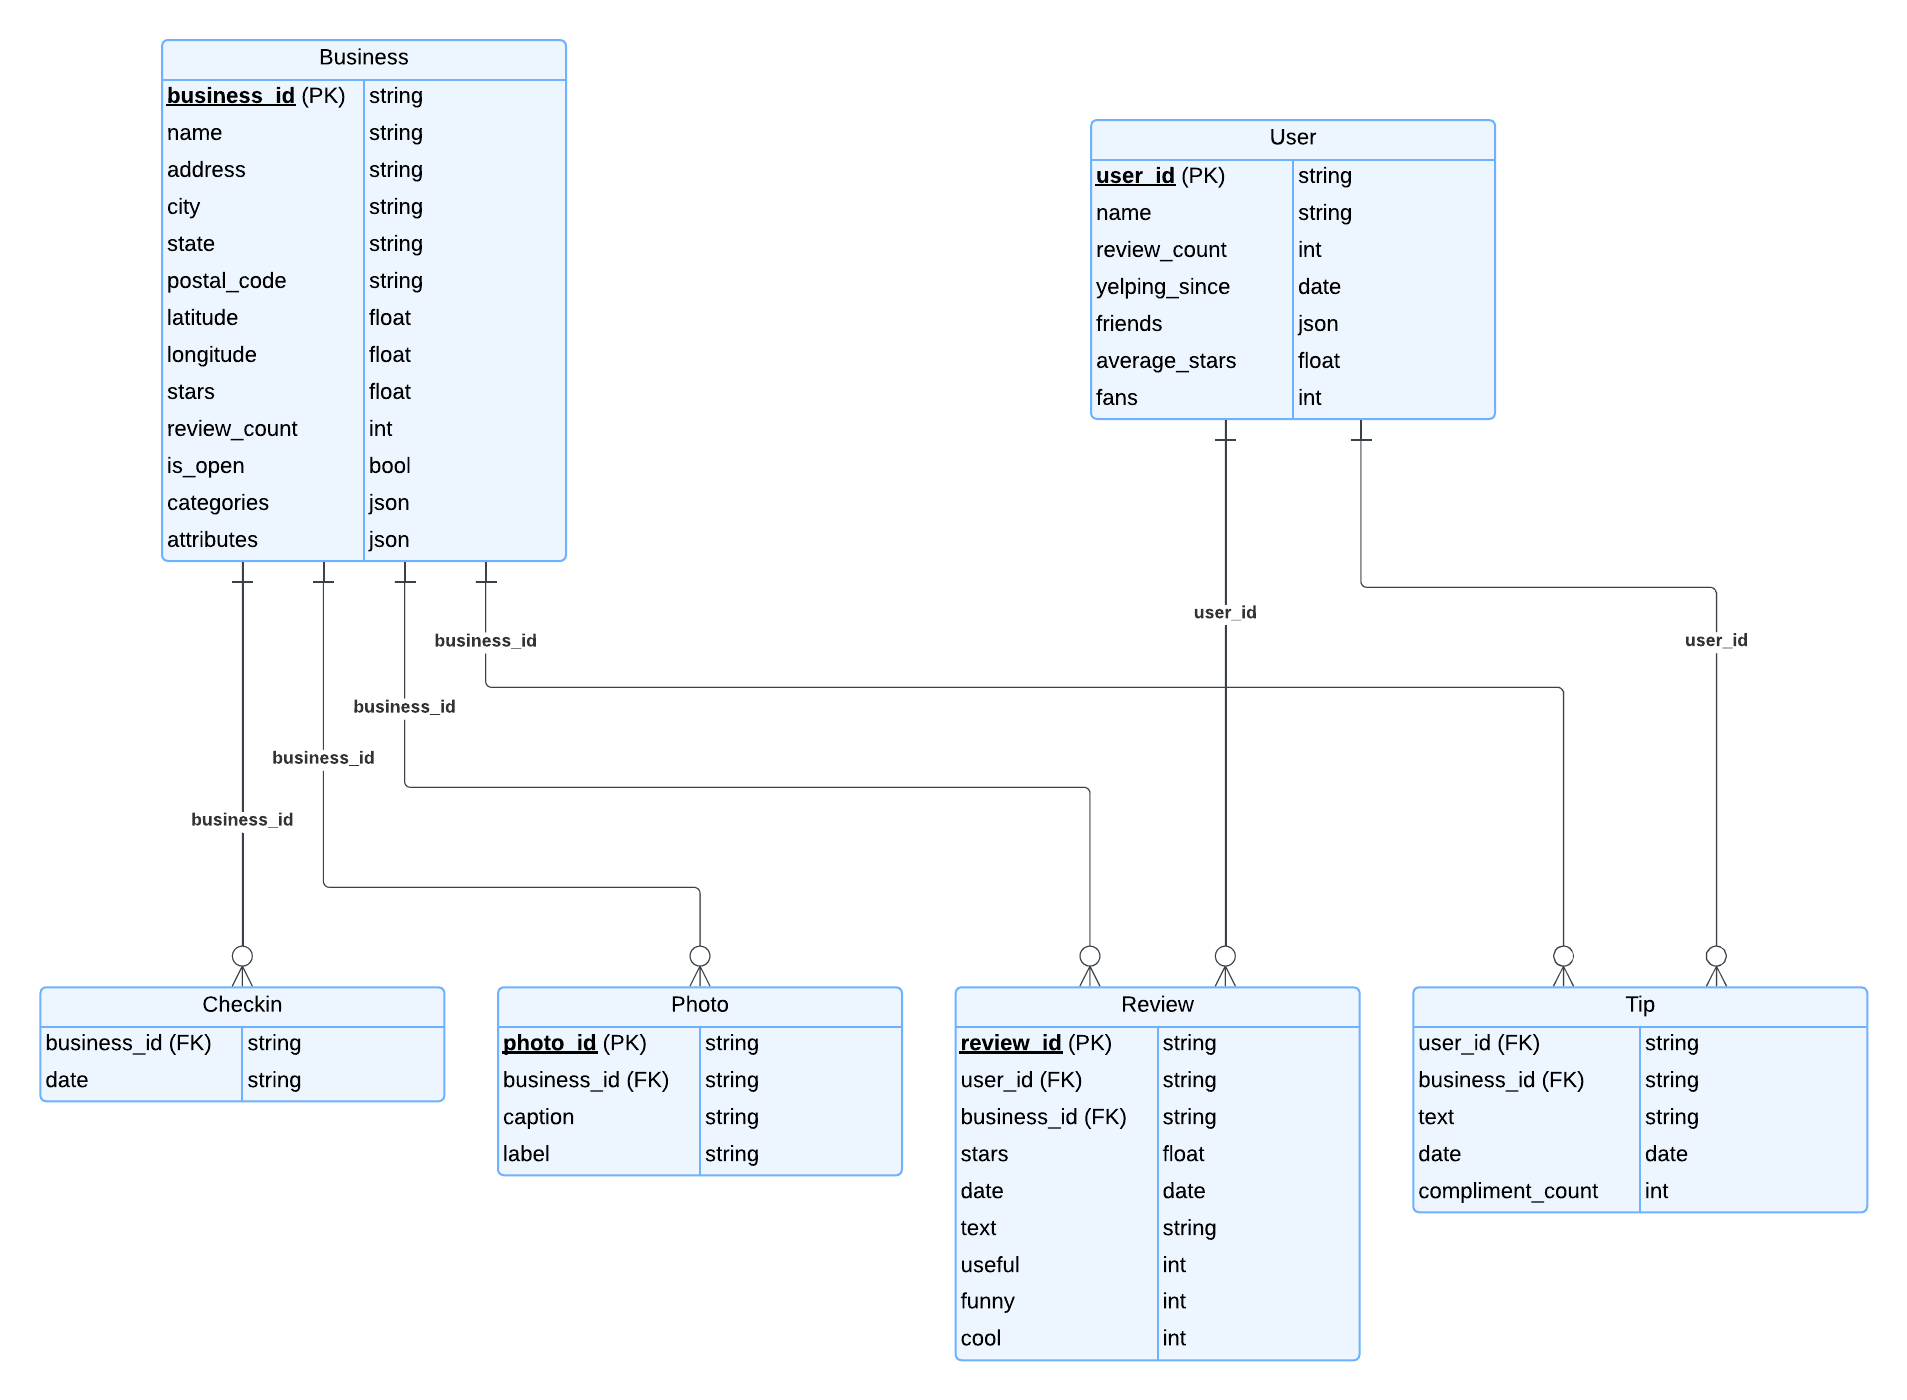
\includegraphics[width=0.8\textwidth]{er-diagram.png} % Change 'image.png' to your image file name
    \caption{ER diagram of Yelp dataset schema and relationships.}
    \label{fig:example} % Label for referencing the figure in the text
\end{figure}


As seen in our ER diagram, the dataset is made up of the following JSON files:
\begin{itemize}
    \item \textbf{business.json}: Business data, location data, attributes, and categories.
    \item \textbf{review.json}: Review text data, \texttt{user\_id} of the review writer, \texttt{business\_id} of the business reviewed, and review attributes and votes.
    \item \textbf{user.json}: User data, attributes, user friend mapping, user metadata.
    \item \textbf{checkin.json}: \texttt{business\_id}, date of check-in.
    \item \textbf{tip.json}: Tip text data, \texttt{user\_id} and \texttt{business\_id}.
    \item \textbf{photo.json}: Photo and \texttt{business\_ids}, photo attributes.
\end{itemize}

Each file is composed of a single object type, one JSON-object per line.


\section{Data Sampling and Truncation Plans}

The Yelp dataset is comprehensive, encompassing millions of records across users, businesses, and reviews. To ensure efficient processing while maintaining representativeness, we applied the following sampling and truncation strategies:

\begin{itemize}
    \item \textbf{Users:} The dataset originally contains several million user records. We sampled approximately 2 million users to reduce storage overhead and computational complexity. This sampling ensures proportional representation across different user activity levels and geographies.
    \item \textbf{Businesses:} All business records were retained without sampling. This allows for a complete representation of businesses across regions and categories.
    \item \textbf{Reviews:} Reviews were filtered based on references to existing users in the \texttt{users} table and businesses in the \texttt{businesses} table. This ensures referential integrity while excluding reviews that belong to users or businesses outside our database.
\end{itemize}